\section{Sistemi lineari ed interazioni tra sistemi}

I sistemi di equazioni differenziali più semplici che possiamo considerare sono i \textbf{sistemi lineari} e dall'analisi matematica sappiamo che possiamo sempre trovare una soluzione, unica, per questo tipo di equazioni, una volta stabilite le condizioni iniziali.
\begin{equation}
	x\in\mathbb{R}^n \qquad \dot{x}=Ax \qquad \Rightarrow \qquad x(t)=\sum_\lambda v_\lambda \ e^{\lambda t}
\end{equation}
Dove $A$ è una matrice quadrata $n\times n$ e $v_\lambda$ è un suo auto vettore di autovalore $\lambda$.\\

La semplicità di queste soluzioni consentono di stimare l'evoluzione di una perturbazione delle condizioni iniziali $\delta x_0$ ad un tempo $t$:
\begin{equation}
	\|\delta x(t)\| \backsimeq |e^{\lambda t}|\ \|\delta x_0\|
\end{equation}
\paragraph{Esponente di Lyapunov}
dove $\lambda$ è detto \textbf{esponente di Lyapunov} e chiaramente se ha parte reale positiva implica che la perturbazione porterà la soluzione a divergere da quella iniziale.

Possiamo inoltre stimare il \textbf{tempo di predicibilità} del modello come il tempo $t^*$ per cui errori piccoli sulle condizioni iniziali non sono più trascurabili:
\begin{equation}
	\|\delta x_0\| \ |e^{\lambda t^*}|\sim1\qquad\Rightarrow\qquad t^*=-\frac{\log\|\delta x_0\|}{\lambda}
\end{equation}

Infine forniamo un modo per definire e stimare l'esponente di Lyapunov: la definizione formale fa uso del concetto di \textbf{flusso di fase} $\Phi^t(x_0)$, mentre la stima è basata sull'idea di misurare ad intervalli regolari $\Delta T$ di quanto divergono due soluzioni e di mediare i vari esponenti di Lyapunov che troviamo "empiricamente":
\begin{equation}
	\lambda=\lim_{\delta\rightarrow0,\ t\rightarrow\infty}\log\|\Phi^t(x_0+\delta x_0)-\Phi^t(x_0)\| \frac{1}{t} \qquad \lambda\backsimeq\frac{1}{N\Delta T}\sum_{k=0}^N \log |\frac{\delta x_k(\Delta T)}{\delta x_k(0)}|
\end{equation} 

\subsection{Perturbazioni del sistema}

Possiamo pensare di perturbare il sistema modificando la matrice che definisce le equazioni differenziali, questo tipo di meccanismo vedremo che può essere interpretato come l'interazione tra più sistemi. Per trattare questo problema poniamoci nella condizione di aver diagonalizzato $A$ e di sommarci una matrice $B$ moltiplicata per un fattore $\epsilon$:
\begin{equation}
	\dot{x}=(\Lambda+\epsilon B)x
\end{equation}
Supponiamo quindi che la soluzione del nuovo sistema sia quella imperturbata moltiplicata per una funzione correttiva $x(t)=e^{\Lambda t}y(t)$ così da poter suddividere il sistema in altre due equazioni differenziali che consentono di stimare gli effetti di perturbazione:
\begin{equation*}
	\begin{gathered}
		\frac{d}{dt}(e^{\Lambda t}y(t))=\Lambda e^{\Lambda t}y(t)+e^{\Lambda t}\dot{y}(t)=(\Lambda+\epsilon B)(e^{\Lambda t}y(t))\\
		\Rightarrow \qquad 
		\begin{cases}
			e^{\Lambda t}\dot{y}(t)=\epsilon Be^{\Lambda t}y(t)\\
			\Lambda x(t)=\Lambda e^{\Lambda t}y(t)
		\end{cases}
	\Rightarrow \dot{y}=e^{-\Lambda t}\epsilon B e^{\Lambda t} y(t)
	\end{gathered}
\end{equation*}
Possiamo quindi procedere ad integrare quest'ultima equazione differenziale:
\begin{equation}
	y(t)-y_0=\epsilon\int_{0}^{t}e^{-\Lambda s} B e^{\Lambda s} y(s)\ ds
\end{equation}
Osserviamo che però l'integrando presenta una dipendenza esplicita da $y$ che però è proprio la variabile che intendiamo stimare. Al fine di riuscire per lo meno a stimare questo integrale approssimiamo $y(t) \backsimeq y_0$, nella fattispecie se consideriamo $\epsilon$ piccolo è chiaro che introdurre approssimazioni di ordine superiore non è necessario poichè $\epsilon$ appare già linearmente nell'intregrando ottenendoci un'approssimazione complessiva di $y(t)$ al prim'ordine.\\
Conviene osservare anche che per $t=0$ la soluzione perturbata, avendo le stesse condizioni iniziali del sistema imperturbato, deve soddisfare $y(0)=x_0$, per cui:
\begin{equation}
	y(t)= x_0+\epsilon\int_{0}^{t}e^{-\Lambda s} B e^{\Lambda s} x_0\ ds + O(\epsilon^2)
\end{equation}
che inserita nella soluzione generale ci consente di ottenere:
\begin{equation}
	x(t)=e^{\Lambda t}y(t)= e^{\Lambda t}x_0+\epsilon\int_{0}^{t}e^{-\Lambda (t-s)} B e^{\Lambda s} x_0\ ds + O(\epsilon^2)
	\label{soluzionePerturbata}
\end{equation}
In ultima battuta possiamo "inglobare" gli elementi non diagonali di $B$ in $\Lambda'=\Lambda+ \epsilon Diag(B)$ e studiare quindi $\hat{B}=B-Diag(B)$. In questo modo la (\ref{soluzionePerturbata}) si riduce ad una serie di integrali indicizzati che compongono la matrice da applicare ad $x_0$:
\begin{equation*}
	\epsilon\int_{0}^{t}e^{-\lambda'_h (t-s)} \hat{B}_{hk} e^{\lambda'_k s}\ ds=\epsilon\frac{e^{\lambda'_ht}-e^{\lambda'_kt}}{\lambda'_k-\lambda'_h}B_{hk}
\end{equation*}
che chiaramente evidenzia una maggiore sensibilità del sistema a perturbazioni se due autovalori tendono ad uguagliarsi.

\subsection{Sistemi interagenti}
Per modellizzare una serie di sistemi interagenti consideriamo una serie di particelle dotate di una dinamica propria ma capaci di influenzarsi a vicenda, in questo caso considereremo che la particella k-esima è influenzata solamente dalla sua precedente mediante una relazione lineare che perturba la sua dinamica propria.
\begin{center}
	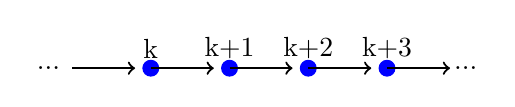
\begin{tikzpicture}
		
		\node[] at (-1.3,0) {...};
		\node[] at (4,0) {...};
		
		\filldraw[fill=blue,draw=blue] (0,0) circle (0.1cm) node[above] {k};
		\filldraw[fill=blue,draw=blue] (1,0) circle (0.1cm) node[above] {k+1};
		\filldraw[fill=blue,draw=blue] (2,0) circle (0.1cm) node[above] {k+2};
		\filldraw[fill=blue,draw=blue] (3,0) circle (0.1cm) node[above] {k+3};
		\draw[->, thick] (0,0) -- (0.8,0);
		\draw[->, thick] (-1,0) -- (-0.2,0);
		\draw[->, thick] (1,0) -- (1.8,0);
		\draw[->, thick] (2,0) -- (2.8,0);
		\draw[->, thick] (3,0) -- (3.8,0);
		
		
	\end{tikzpicture}

    \begin{equation}
    	\dot{x}_k=F(x_k)+\epsilon Bx_{k-1} \qquad x\in\mathbb{R}^n
    	\label{diffeqinteragenti}
   \end{equation}	
\end{center} 
Come vedremo questo tipo di sistemi può rappresentare per esempio il moto delle macchine sulla strada, dove ogni particella è una macchina e regola la sua velocità in base al comportamento della macchina che ha subito davanti, ma anche una serie di neuroni soggetti ad un impulso esterno che è direttamente fornito dal neurone precedente.\\

Chiediamoci ora se è possibile trasmettere perturbazioni nel sistema da una particella ad un'altra e se si quale vaore di $\epsilon$ lo consente. Osserviamo quindi che la nostra richiesta è del tutto analoga alla richiesta di trasmettere un'onda nel sistema, per cui se definiamo un parametro $\Delta$ che quantifica la "distanza" tra due particelle allora la soluzione deve essere nella forma:
\begin{equation}
	x_k(t)=u(k\Delta - t)
	\label{conditioonda}
\end{equation}
Chiaramente se chiamiamo $u^*$ un preciso valore della soluzione questo è univocamente determinato dal suo argomento che però è dipendente sia dall'indice della particella considerata sia dal tempo, per cui per mantenere l'argomento della funzione costante al variare del tempo dovrò anche variare k permettendo così a $u^*$ di propagarsi nel sistema come un fronte d'onda. \\Solitamente la ricerca di questa soluzione particolare è giustificata dall' osservazione di dinamiche ondulatorie nel sistema.\\

Procediamo quindi sostituendo la (\ref{conditioonda}) nella (\ref{diffeqinteragenti}) in maniera tale da ottenere una \textbf{equazione differenziale con ritardo}, questo tipo di equazioni non è solitamente di facile risoluzione poichè presentano un numero di gradi di libertà non numerabile dovuto alla dipendenza della derivata dalle condizioni ad un tempo precedente $t'-\Delta$. Nella fattispecie osserviamo che $x_{k-1}=u((k-1)\Delta+t)$ ed introducendo la variabile $t'=k\Delta-t$ abbiamo:
\begin{equation*}
		\dot{x}_k=\dot{u}=F(u)+\epsilon Bu(k\Delta+t-\Delta)
\end{equation*}
\paragraph{Equazione differenziale con ritardo}
\begin{equation}
	\dot{u}=F(u)+\epsilon Bu(t'-\Delta) \label{eqdiffritardo}
\end{equation}
Se a questo punto la (\ref{eqdiffritardo}) risulta lineare o è linearizzabile possiamo cercare una sua soluzione nella forma esponenziale dipendente degli autovalori di una matrice. 
\begin{equation*}
	u(t)=\sum v_\lambda e^{\lambda t}\qquad \Rightarrow \qquad  \lambda v_\lambda = (A+\epsilon Be^{-\Delta\lambda})v_\lambda
\end{equation*}
Inserendo la ipotizzata soluzione nella (\ref{eqdiffritardo}) scopriamo che gli autovalori sono della matrice $A+\epsilon Be^{-\Delta\lambda}$, per è chiaro dall'algebra lineare che possiamo trovarli e quindi risolvere l'equazione differenziale, tramite la risluzione del polinomio caratteristico dato dal determinate della matrice che abbiamo ottenuto:
\begin{equation}
	\det(\lambda I-A-\epsilon Be^{-\Delta \lambda})=0
\end{equation}

Consideriamo ora le particelle non più collegate in maniera sequenziale ma a formare una grafo dove ogni particella è un nodo collegata ad altri con dei link che consentano di interagire in entrambe le direzioni. Possiamo definire la \textbf{matrice di adiacenza} $A_{ij}$ che assume il valore $1$ se tra la particella i-esima e j-esima vi è un link e "0" altrimenti. Così facendo la (\ref{diffeqinteragenti})
diventa:
\begin{equation}
		\dot{x}_k=F(x_k)+\epsilon \sum A_{kh} x_h
\end{equation}
Questa tipologia di equazioni differenziali può essere ulteriormente modificato affinchè le interazioni, che possono essere viste come scambi di una certa quantità tra una particella ed un'altra, abbiano un senso più fisico, ossia che la quantità scambiata, in analogia con l'impulso, sia conservata. Per far ciò introduciamo il vettore $D_i=\sum A_{ij}$ che assume il valore esatto di link che possiede un determinato nodo, questa matrice ci consente di aggiungere un termine di "conservazione":
\begin{equation}
	\dot{x}_k=F(x_k)+\epsilon \sum( A_{kh} x_h-\delta_{hk}D_kx_k)
\end{equation}
\paragraph{Matrice laplaciana}
Il termine di interazione così costruito trasferisce una quantità dinamica alle particelle collegate attraverso la matrice di adiacenza e ne sottrae una pari quantità alla particella k-esima, attraverso il vettore $D_k$, così che ne complesso si abbia conservazione. Il termine complessivo di interazione prende quindi il nome di \textbf{matrice laplaciana}:
\begin{equation}
	L_{kh}=-( A_{kh}-\delta_{hk}D_k)
\end{equation}
Queste matrici svolgono il ruolo discreto dell'operatore laplciano e risultano dunque estremamente utili per lo studio dei sistemi interagenti, delle loro numerose proprietà ne citiamo le più importanti:
\begin{itemize}
	\item L è simmetrica
	\item Se L ha più di un autovalore nullo il grafo è separabile in due sottosistemi distinti
	\item Se il grafo non è separabile ho tutti autovalori positivi tranne uno nullo che ha sempre l'autovettore associato $v_\lambda=(1,1,1,...)$.
\end{itemize}
\subsection{Sincronizzazione di sistemi intergaenti}
\begin{center}
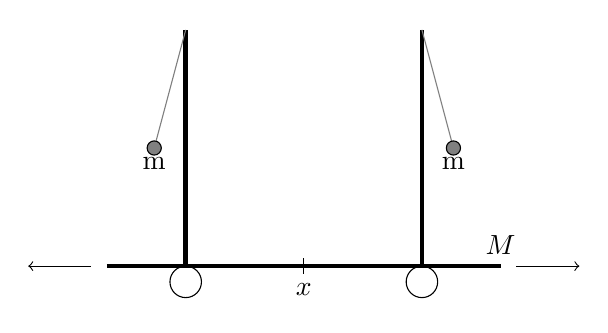
\begin{tikzpicture}
	\draw[ultra thick] (0,0) -- (5,0) node[above] {$M$};
	\draw (1,-0.2) circle (0.2cm);
	\draw (4,-0.2) circle (0.2cm);
	\draw[<-] (-1,0) -- (-0.2,0);
	\draw[->] (5.2,0) -- (6,0);
	\draw (2.5,0.1) -- (2.5,-0.1)  node[below] {$x$};
	\draw[ultra thick] (1,0) -- (1,3);
	\draw[ultra thick] (4,0) -- (4,3);
	\draw[draw=gray] (1,3) -- (0.6,1.5);
	\filldraw[fill=gray] (0.6,1.5) circle (0.09cm) node[below] {m};
		\draw[draw=gray] (4,3) -- (4.4,1.5);
	\filldraw[fill=gray] (4.4,1.5) circle (0.09cm) node[below] {m};
	
\end{tikzpicture}
\end{center}
Per analizzare il problema della sincronizzazione proviamo a studiare il sistema meccanico rappresentato sopra, costituito da due pendoli di massa $m$ legati ad un filo di lunghezza $l$ e vincolati su una base basculante di massa $M$, si osserva sperimentalmente che questo tipo di sistema si sincronizza in maniera tale che, seppur partendo da fasi differenti, le oscillazioni dei due pendoli tendano ad un moto sincrono controfase. Per cominciare scriviamo la lagrangiana del sistema:
\begin{equation}
	\mathcal{L}=\frac{M}{2}\dot{x}^2+\frac{m}{2}(2\dot{x}^2+\dot{\theta_1}^2l^2+\dot{\theta_2}^2l^2+2\dot{x}l(\dot{\theta_1}\cos\theta_1+\dot{\theta_2}\cos\theta_2))+mgl(\cos\theta_1+\cos\theta_2)
\end{equation}
conoscendo quest'ultima possiamo descrivere l'evoluzione dinamica dei pendoli, osserviamo però che questo sistema, nelle ipotesi ideali che stiamo assumendo implicitamente, non può sincronizzarsi, infatti una proprietà dei sistemi dinamici \textit{Hamiltoniani} è la reversibilità che verrebbe a mancare se avvenisse la sincronizzazione: infatti giunti alla condizione di moto sincrono non si sarebbe più in grado si risalire alle condizioni iniziali.\\
Siamo infatti costretti a considerare gli attriti così da non studiare più un sistema reversibile, per cui procediamo in primis considerando il regime delle piccole oscillazioni:
\begin{equation}
	\mathcal{L}_{po}=\frac{M}{2}\dot{x}^2+\frac{m}{2}(2\dot{x}^2+\dot{\theta_1}^2l^2+\dot{\theta_2}^2l^2+2\dot{x}l(\dot{\theta_1}+\dot{\theta_2}))-\frac{mgl}{2}(\theta_1^2+\theta_2^2)
\end{equation}
Osserviamo che $x$ è una coordinata ciclica per cui è il suo momento associato è un integrale primo del moto da cui abbiamo $\dot{x}=-l\frac{m}{2m+M}(\dot{\theta_1}+\dot{\theta_2})$ che ci consente di ridurre i gradi di livertà del problema e di ricondurci ad una lagrangiana data da sole forme quadratiche, infatti se chiamiamo $a=\frac{m}{2m+M}$ tramite qualche passaggio algebrico abbiamo:
\begin{equation*}
   \begin{gathered}
   	\mathcal{L}_{po}=l^2\frac{m}{2}(1-a)(\dot{\theta_1}^2+\dot{\theta_2}^2)+2ml^2a(a-1)\dot{\theta_1}\dot{\theta_2}-\frac{mgl}{2}(\theta_1^2+\theta_2^2)\\
   	\mathcal{L}_{po}=l^2\frac{m}{2}(1-a)
   	\begin{pmatrix}
   		\dot{\theta_1} \\
   		\dot{\theta_2}
   	\end{pmatrix}
   \begin{pmatrix}
   	1 & -2a \\
   	-2a & 1
   \end{pmatrix} 
   \begin{pmatrix}
   	\dot{\theta_1} \\
   	\dot{\theta_2}
   \end{pmatrix}
   -\frac{mgl}{2}
   \begin{pmatrix}
   	\theta_1 \\
   	\theta_2
   \end{pmatrix}
   I
   \begin{pmatrix}
   	\theta_1 \\
   	\theta_2
   \end{pmatrix}
   \end{gathered}	
\end{equation*}
utilizzando le equazioni di eulero-lagrange otteniamo il sistema di equazioni differenziali:
\begin{equation*}
	\begin{gathered}
		l^2m(1-a)
		\begin{pmatrix}
			1 & -2a \\
			-2a & 1
		\end{pmatrix}
	\begin{pmatrix}
		\ddot{\theta_1} \\
		\ddot{\theta_2}
	\end{pmatrix}
    =-mgl
    \begin{pmatrix}
    	\theta_1 \\
    	\theta_2
    \end{pmatrix}
	\end{gathered}	
\end{equation*}
introduciamo un termine d'attrito:
\begin{equation*}
	\begin{gathered}
		l^2m(1-a)
		\begin{pmatrix}
			1 & -2a \\
			-2a & 1
		\end{pmatrix}
		\begin{pmatrix}
			\ddot{\theta_1} \\
			\ddot{\theta_2}
		\end{pmatrix}
		=-\gamma
			\begin{pmatrix}
			\ddot{\theta_1} \\
			\ddot{\theta_2}
		\end{pmatrix}
		-mgl
		\begin{pmatrix}
			\theta_1 \\
			\theta_2
		\end{pmatrix}
	\end{gathered}	
\end{equation*}
Se diagonaliziamo la matrice metrica dell'energia cinetica troviamo due autovettori con due auto valori, le combinazioni lineari delle soluzioni del sistema secondo questi due autovettori ci danno la generica soluzione per cui:
\begin{itemize}
	\item $\lambda=1-2a$ con $v_{\lambda}=(1,1)$, che da un sistema oscillante in fase che è descritto dall'equazione:
	\begin{equation*}
			\begin{pmatrix}
				\ddot{\theta_1} \\
				\ddot{\theta_2}
			\end{pmatrix}
			=-\frac{\gamma}{l^2m(1-a)(1-2a)}
			\begin{pmatrix}
				\ddot{\theta_1} \\
				\ddot{\theta_2}
			\end{pmatrix}
			-\frac{g}{l(1-a)(1-2a)}
			\begin{pmatrix}
				\theta_1 \\
				\theta_2
			\end{pmatrix}
	\end{equation*}
In questo caso poichè $a=\frac{m}{2m+M}$ per $M\rightarrow0$ abbiamo che $a\rightarrow\frac{1}{2}$ il termine dissipativo diventa infinitamente grande, per cui questa soluzione se presente si dissipa molto rapidamente se la massa della base è molto piccola.
\item $\lambda=1+2a$ con $v_{\lambda}=(1,-1)$, che da un sistema oscillante in controfase che è descritto dall'equazione:
\begin{equation*}
	\begin{pmatrix}
		\ddot{\theta_1} \\
		\ddot{\theta_2}
	\end{pmatrix}
	=-\frac{\gamma}{l^2m(1-a)(1+2a)}
	\begin{pmatrix}
		\ddot{\theta_1} \\
		\ddot{\theta_2}
	\end{pmatrix}
	-\frac{g}{l(1-a)(1+2a)}
	\begin{pmatrix}
		\theta_1 \\
		\theta_2
	\end{pmatrix}
\end{equation*}
Con lo stesso ragionamento del punto precedente osserviamo che il termine dissipativo non cresce rapidamente come nel caso in fase il che consente a questo modo di manifestarsi nella dinamica del sistema che risulterà quindi sincronizzato.
\end{itemize} 